\documentclass[12pt,letterpaper]{article}
\usepackage[utf8]{inputenc}
\usepackage[spanish]{babel}
\usepackage{graphicx}
\usepackage[left=2cm,right=2cm,top=2cm,bottom=2cm]{geometry}
\usepackage{graphicx} % figuras
% \usepackage{subfigure} % subfiguras
\usepackage{float} % para usar [H]
\usepackage{amsmath}
%\usepackage{txfonts}
\usepackage{stackrel} 
\usepackage{multirow}
\usepackage{enumerate} % enumerados
\renewcommand{\labelitemi}{$-$}
\renewcommand{\labelitemii}{$\cdot$}
% \author{}
% \title{Caratula}
\begin{document}

% Fancy Header and Footer
% \usepackage{fancyhdr}
% \pagestyle{fancy}
% \cfoot{}
% \rfoot{\thepage}
%

% \usepackage[hidelinks]{hyperref} % CREA HYPERVINCULOS EN INDICE

% \author{}
\title{Caratula}

\begin{titlepage}
\begin{center}
\large{UNIVERSIDAD PRIVADA-DE-TACNA}\\
\vspace*{-0.025in}
\begin{figure}[htb]
\begin{center}

\includegraphics[width=8cm]{./Imagenes/logo}
\end{center}
\end{figure}
\vspace*{0.15in}
INGENIERIA DE SISTEMAS  \\

\vspace*{0.5in}
\begin{large}
TITULO:\\
\end{large}

\vspace*{0.1in}
\begin{Large}
\textbf{Trabajo Final de Unidad} \\
\end{Large}

\vspace*{0.3in}
\begin{Large}
\textbf{CURSO:} \\
\end{Large}

\vspace*{0.1in}
\begin{large}
BASE DE DATOS II\\
\end{large}

\vspace*{0.3in}
\begin{Large}
\textbf{DOCENTE(ING):} \\
\end{Large}

\vspace*{0.1in}
\begin{large}
 Patrick Cuadros Quiroga\\
\end{large}

\vspace*{0.2in}
\vspace*{0.1in}
\begin{large}
Integrantes: \\
\begin{flushleft}
Orlando Antonio Acosta Ortiz		\hfill	(2015052775) \\
Orestes Ramirez Ticona              \hfill  (2015053236) \\
Nilson Laura Atencio     			\hfill 	(2015053846) \\
Roberto Zegarra Reyes 				\hfill 	(2010036175) \\
Richard Cruz Escalante 				\hfill 	(2013047247) \\
Wilfredo Vilca Chambilla    \hfill 	(2006028540) \\
\end{flushleft}
\end{large}
\end{center}

\end{titlepage}


\tableofcontents % INDICE
\thispagestyle{empty} % INDICE SIN NUMERO
\newpage
\setcounter{page}{1} % REINICIAR CONTADOR DE PAGINAS DESPUES DEL INDICE

\section{INFORMACIÓN GENERAL} 

\begin{itemize}
\subsection{Objetivos:}
	\item Tener conocimiento acerca de Pruebas Unitarias en C Sharp

\subsection{Equipos, materiales, programas y recursos utilizados:}
	\item Computadora con sistema operativo Windows 10.
	\item Microsoft Visual Studio 2017
	\item Microsoft SQL Server 2016
	\item Net Framework 4.6.1
	\item Base de datos SchoolDB

\end{itemize}
\section{MARCO TEORICO} 
\begin {itemize}
\subsection{Entity Framework}
	\item Entity Framework (EF) es un mapeador relacional de objetos (O/RM) probado y probado para .NET con muchos años de desarrollo y estabilización de características.\\
Es la tecnología de acceso a datos recomendada por Microsoft para nuevas aplicaciones.\\	
	\item Como O/RM, EF reduce la discrepancia de impedancia entre los mundos relacionales y orientados a objetos, permitiendo a los desarrolladores escribir aplicaciones que interactúan con datos almacenados en bases de datos relacionales utilizando objetos .NET de tipo fuerte que representan el dominio de la aplicación y eliminando la necesidad para una gran parte del código de "plumbing" de acceso a datos que normalmente necesitan escribir.\\
	\item EF implementa muchas características populares de O/RM:\\
	- Mapeo de clases de entidad POCO que no dependen de ningún tipo de EF\\
	- Seguimiento automático de cambios\\
	- Resolución de identidad y Unidad de Trabajo.\\
	- Carga ansiosa, perezosa y explícita.\\
	- Traducción de consultas fuertemente tipadas utilizando LINQ \\
	- Capacidades de mapeo enriquecidas, incluyendo soporte para:\\
	\subitem - Relaciones uno a uno, uno a muchos y muchos a muchos\\
	\subitem - Herencia (tabla por jerarquía, tabla por tipo y tabla por clase concreta)\\
	\subitem - Tipos complejos\\
	\subitem - Procedimientos almacenados\\
	\newline
	- Un diseñador visual para crear modelos de entidad.\\
	- Una experiencia de "Código Primero" para crear modelos de entidad al escribir código.\\
	- Los modelos pueden generarse a partir de bases de datos existentes y luego editarse manualmente, o pueden crearse desde cero y luego usarse para generar nuevas bases de datos.\\
	- Integración con modelos de aplicaciones de .NET Framework, incluido ASP.NET, y mediante enlace de datos, con WPF y WinForms.\\
	- Conectividad de base de datos basada en ADO.NET y numerosos proveedores disponibles para conectarse a SQL Server, Oracle, MySQL, SQLite, PostgreSQL, DB2, etc.\\
	\newpage
\subsection {Pruebas Unitarias}
\item Una prueba unitaria se utiliza para comprobar que un método concreto del código de producción funciona correctamente, probar las regresiones o realizar pruebas relacionadas (buddy) o de humo. Una prueba por orden se utiliza para ejecutar otras pruebas en un orden especificado. 
\end{itemize}

\section{PROCEDIMIENTO} 
Parte 1: Consultando Datos
\begin{itemize}
	\item Crear un proyecto de pruebas a nuestra solución.
	\item Dentro de la clase, agregamos el siguiente metodo ObtenerAlEstudianteConIDUno.
	\begin{figure}[htb]
\begin{center}
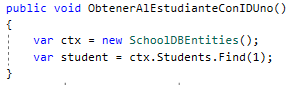
\includegraphics[width=12cm]{./Imagenes/1-1}
\end{center}
\end{figure}
	\item Agregamos el siguiente metodo BuscarAlPrimerEstudianteConElNombreBill.
\begin{figure}[htb]
\begin{center}
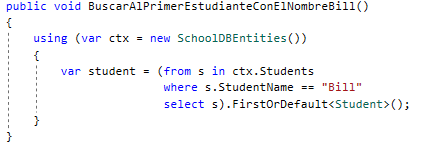
\includegraphics[width=12cm]{./Imagenes/1-2}
\end{center}
\end{figure}
	\item Agregamos el siguiente metodo BuscarEstudiantesAgrupadosPorEstandar.
\begin{figure}[htb]
\begin{center}
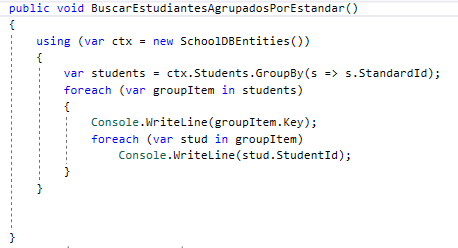
\includegraphics[width=12cm]{./Imagenes/1-3}
\end{center}
\end{figure}
	\item Agregamos el siguiente metodo ObetenerListadoDeEstudiantesOrdenadosPorNombre.
\begin{figure}[htb]
\begin{center}
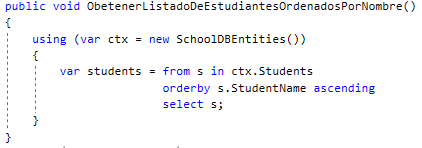
\includegraphics[width=12cm]{./Imagenes/1-4}
\end{center}
\end{figure}
	\item Agregamos el siguiente metodo BuscarTodosLostudiantesConElEstandarUno.
\begin{figure}[htb]
\begin{center}
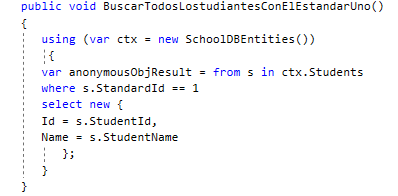
\includegraphics[width=12cm]{./Imagenes/1-5}
\end{center}
\end{figure}
\end{itemize}
Parte 2: Guardando Datos
\begin{itemize}
	\item Agregar al proyecto de pruebas una clase de pruebas TestUnit02, agregar el método
InsertarEstudianteSatisfactoriamente, tomar como referencia el siguiente código.
	\begin{figure}[htb]
\begin{center}
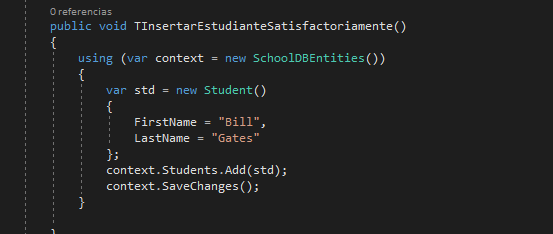
\includegraphics[width=12cm]{./Imagenes/1-6}
\end{center}
\end{figure}
	\item Agregar el método ActualizarElPrimerEstudianteSatisfactoriamente, tomar como referencia el siguiente
código.
\begin{figure}[htb]
\begin{center}
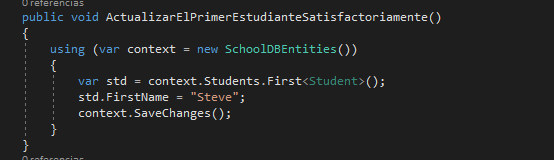
\includegraphics[width=12cm]{./Imagenes/1-7}
\end{center}
\end{figure}
	\item Agregar el método EliminarElPrimerEstudianteSatisfactoriamente, tomar como referencia el siguiente código.
\begin{figure}[htb]
\begin{center}
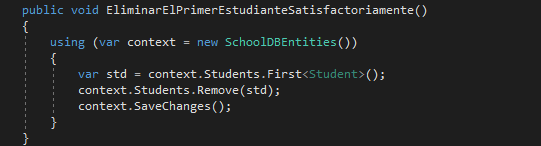
\includegraphics[width=12cm]{./Imagenes/1-8}
\end{center}
\end{figure}
	\item Agregar el método: AgregarTresEstudiantesSatisfactoriamente, tomar como referencia el siguiente código:

\begin{figure}[htb]
\begin{center}
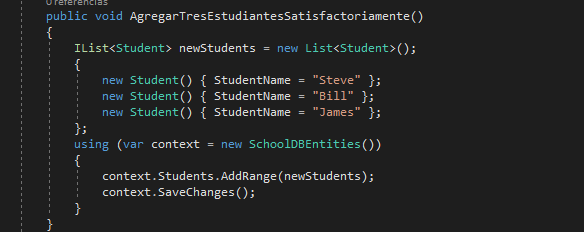
\includegraphics[width=12cm]{./Imagenes/1-9}
\end{center}
\end{figure}
	\item Finalmente agregar el método de pruebas: EliminarTresEstudiantesSatisfactoriamente, tomar como referencia el siguiente código:
\begin{figure}[htb]
\begin{center}
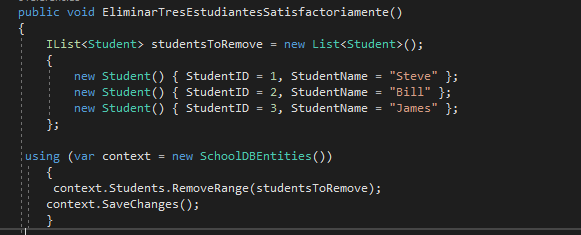
\includegraphics[width=12cm]{./Imagenes/1-10}
\end{center}
\end{figure}
\end{itemize}






\section{ANALISIS E INTERPRETACION DE RESULTADOS} 
-Al compilar el proyecto de prueba, las pruebas aparecen en el Explorador de pruebas. Si el Explorador de pruebas no está visible, elija Prueba en el menú de Visual Studio, elija Ventanas y, después, Explorador de pruebas.
-Se puede elegir Ejecutar todas para ejecutar todas las pruebas o bien Ejecutar para elegir un subconjunto de pruebas que se desea ejecutar. Después de ejecutar un conjunto de pruebas, aparecerá un resumen de la serie de pruebas en la parte inferior de la ventana Explorador de pruebas. Seleccione una prueba para ver los detalles de esa prueba en el panel inferior. 
\begin{itemize}
	\item Al compilar el proyecto de prueba.
	\begin{figure}[htb]
\begin{center}
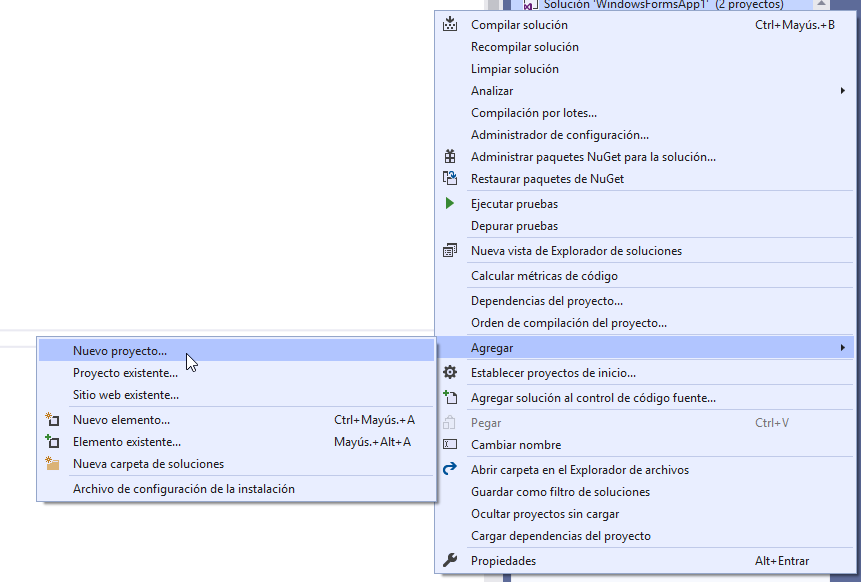
\includegraphics[width=12cm]{./Imagenes/imp1}
\end{center}
\end{figure}
	\item Explorador de pruebas.
\begin{figure}[htb]
\begin{center}
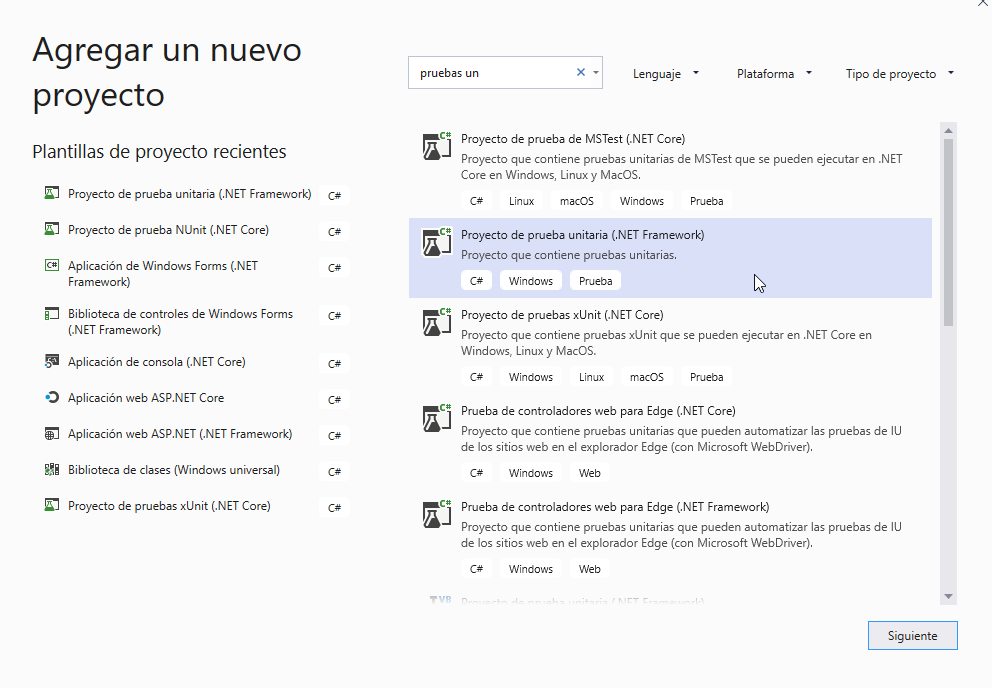
\includegraphics[width=12cm]{./Imagenes/imp2}
\end{center}
\end{figure}
\end{itemize}

\section{REFERENCIAS}

\begin{itemize}
	\item [[ 1]]  Torres, M. (2012). PROGRAMACION ORIENTADA A OBJETOS CON VISUAL BASIC 2012. Editorial Macro. Pág. 370[[1]
 	\item   [[ 2]] Elman, J. y Lavin, M. (2014). Django ligero: utilizando REST, WebSockets y Backbone. Editor "O'Reilly Media, Inc. Pág. 61
	\item  [[ 3]]  Hugon, J. (2014). C\# 5: desarrolle aplicaciones Windows con Visual Studio 2013. Ediciones ENI. Pág. 269
\end{itemize}

\section{REFERENCIAS} 


\end{document}
